% **************************************************
% Document class
% **************************************************

\documentclass[
	a4paper,
	12pt,
	bibtotoc,
	listof=totoc,
	titlepage
]{scrartcl}


% **************************************************
% Settings
% **************************************************

\usepackage{settings}


% **************************************************
% Variables
% **************************************************

\newcommand*{\getUniversity}{Hochschule für angewandte Wissenschaften München}
\newcommand*{\getFaculty}{Fakultät für Geoinformation}
\newcommand*{\getTitle}{Untersuchung der Implementierung von Contraction Hierarchies in Straßennetzwerken}
\newcommand*{\getAuthor}{Daniel Holzner}
\newcommand*{\getMatriculationNumber}{26576714}
\newcommand*{\getCourse}{Geoinformatik und Navigation}
\newcommand*{\getDoctype}{Bachelorarbeit}
\newcommand*{\getSupervisor}{Prof. Dr. Thomas Abmayr}
\newcommand*{\getSubmissionDate}{\today}

% **************************************************
% Custom commands
% **************************************************
\newcommand*{\zB}{z.\,B. } % Non-breaking z.B.
\newcommand*{\dH}{d.\,h. } % Non-breaking d.h.
\newcommand*{\ua}{u.\,a. } % Non-breaking u.a.


% **************************************************
% PDF Metadata
% **************************************************

\hypersetup{
	pdftitle = \getTitle,
	pdfauthor = \getAuthor,
	pdfsubject = \getDoctype
	pdfkeywords = {Bachelorarbeit, Informatik}
}


% **************************************************
% Content
% **************************************************

\begin{document}

\titlehead{
	\begin{flushright}
		
\includegraphics[width=50mm]{logos/university_logo}
	\end{flushright}
	\begin{center}
		{\Large \getUniversity}\\
		{\large \getFaculty}
		\vspace*{10mm}
	\end{center}
}

\subject{\getDoctype\ zum Thema:}

\title{\vspace{-10mm} \getTitle}

\subtitle{Zur Erlangung des akademischen Grades Bachelor of Science}

\author{}

\date{}

\publishers{
	\parbox{\textwidth}{
		\vspace*{40mm}
		\large
		\begin{tabularx}{0.8\textwidth}{lX}
			\textbf{Vorgelegt von:} & \getAuthor \\[0.7em]
			\textbf{Matrikelnummer:} & \getMatriculationNumber \\[0.7em]
			\textbf{Studiengang:} & \getCourse \\[0.7em]
			\textbf{Betreuer:} & \getSupervisor \\[0.7em]
			\textbf{Abgabedatum:} & \getSubmissionDate \\[0.7em]
		\end{tabularx}
	}
}\normalsize

\maketitle

\begin{abstract}

\section*{Abstract}
Lorem ipsum dolor sit amet, consetetur sadipscing elitr, sed diam nonumy eirmod tempor invidunt ut labore et dolore magna aliquyam erat, sed diam voluptua. At vero eos et accusam et justo duo dolores et ea rebum. Stet clita kasd gubergren, no sea takimata sanctus est Lorem ipsum dolor sit amet. Lorem ipsum dolor sit amet, consetetur sadipscing elitr, sed diam nonumy eirmod tempor invidunt ut labore et dolore magna aliquyam erat, sed diam voluptua. At vero eos et accusam et justo duo dolores et ea rebum. Stet clita kasd gubergren, no sea takimata sanctus est Lorem ipsum dolor sit amet.

\end{abstract}

\tableofcontents

\clearpage
\listoffigures

\clearpage
\listoftables

\clearpage
\lstlistoflistings

\clearpage
\section*{Abkürzungsverzeichnis\markboth{Abkürzungsverzeichnis}{}}
\addcontentsline{toc}{section}{Abkürzungsverzeichnis}

\begin{acronym}[CI]

    \acro{CHs}[CHs]{Contraction Hierarchies}
    \acro{OSM}[OSM]{OpenStreetMap}
    \acro{PQ}[PQ]{Vorrangwarteschlange (eng. Priority Queue)}
\end{acronym}

\clearpage
\section{Einleitung}

Im Folgenden wird beispielhaft gezeigt, wie Zitate, Bilder, Tabellen oder Quellcode in die Arbeit eingefügt werden können.

\subsection{Zitate}
Menschen, die mit ihrem IQ prahlen, sind Versager (\cite[S. 99]{hawking_1999}).

\subsection{Bilder}
\begin{figure}[H]
    \centering
    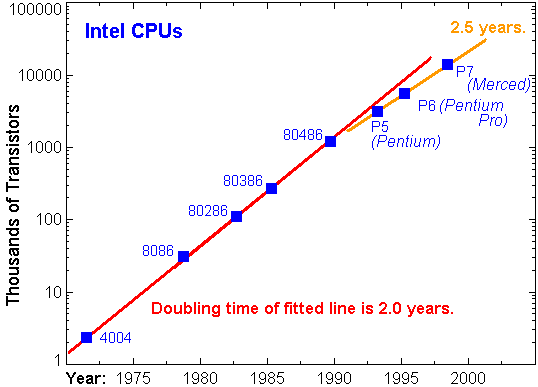
\includegraphics[width=0.5\textwidth]{figures/figure_example.png}
    \caption{Mooresches Gesetz}
\end{figure}

\subsection{Tabellen}
\begin{table}[H]
    \centering
    \begin{tabular}[H]{l|l|l}
        Bezeichnung   & Kerne & TDP   \\
        \hline
        Intel Core i5 & 6     & 111 W \\
        \hline
        AMD Ryzen 7   & 8     & 178 W \\
    \end{tabular}
    \caption{Prozessoren}
\end{table}


\subsection{Quellcode}
\begin{lstlisting}[language=java, caption=Hello World in Java, captionpos=b]
    class HelloWorld {
        public static void main(String[] args) {
            // Display the string.y
            System.out.println("Hello World!");
        }
    }
\end{lstlisting}


\clearpage
\section{Schlussbetrachtung}

Lorem ipsum dolor sit amet, consetetur sadipscing elitr, sed diam nonumy eirmod tempor invidunt ut labore et dolore magna aliquyam erat, sed diam voluptua. At vero eos et accusam et justo duo dolores et ea rebum. Stet clita kasd gubergren, no sea takimata sanctus est Lorem ipsum dolor sit amet. \\

Lorem ipsum dolor sit amet, consetetur sadipscing elitr, sed diam nonumy eirmod tempor invidunt ut labore et dolore magna aliquyam erat, sed diam voluptua. At vero eos et accusam et justo duo dolores et ea rebum. Stet clita kasd gubergren, no sea takimata sanctus est Lorem ipsum dolor sit amet.

\clearpage
\printbibliography

\clearpage
\begin{abstract}

\section*{Selbstständigkeitserklärung}
Hiermit erkläre ich, dass ich die vorliegende Arbeit selbstständig und ohne fremde Hilfe verfasst und keine anderen Hilfsmittel als die angegebenen verwendet habe. \\

München, den \today
\begin{figure}[H] 
  
\includegraphics[width=0.17\textwidth]{logos/signature.png}
\end{figure}

\end{abstract}

\end{document}